\documentclass[10pt]{extarticle} % article doctype, possible font size range from 8pt to 20pt with not all being avaiable.
\setcounter{secnumdepth}{4} % Max. section depth, e.g. 3 means 4.1.1 is possible but not 4.1.1.2
\title{\huge Technical Design Document MaramaUU Editor}
\author{Tim Hintzbergen, Wilbert Schepenaar, <nextname>    \\s1097561, s1094484, <nextcode>
\\\\ICTGPb
\\Wilco Moerman}
\date{May 8th, 2018 <TODO>}

% include packages
\usepackage{graphicx}
\usepackage{caption}
\usepackage{mathabx}
\usepackage{wrapfig}
\usepackage[margin=1.0in]{geometry} % Sets page margin, 2.0in is default.
\usepackage{titlesec}
\usepackage{hyperref}

% custom commands
\newcommand{\myparagraph}[1]{\paragraph{#1}\mbox{}\\} % Without \mbox{} all newlines will be ignored, making the first sentence appear on the same line as a paragraph title.
\newcommand{\code}[1]{\texttt{#1}} % monospace text for code examples.

\DeclareCaptionFormat{cancaption}{#1#2#3\par} % Normal format actually
\DeclareCaptionLabelFormat{cancaptionlabel}{#1}
\captionsetup[figure][number]{format=cancaption,labelformat=cancaptionlabel}
\graphicspath { {images/} }
\begin{document}
    \maketitle
    \thispagestyle{empty}
    \newpage
    %------------------------------------------------------------------------------------------------------------------------------------------------------- Introduction
    \newpage
    \setcounter{page}{1}
    \section {Introduction}
    This document contains all technical aspects of the product regarding the Editor.
    It describes the requirements, the architecture, the design choices and the epics.
    The requirements talk about all functional and non-functional requirements of the product.
    The architecture explains the form of the product, offers a clear overview and talks about some minute details.
    The list of design choices illustrates and defend the various choices that have been made during the design and construction of the product.
    Finally the epics list all coherent components of the product and their submodules
    \newpage

    \tableofcontents{}
    \newpage

    %------------------------------------------------------------------------------------------------------------------------------------------------------- Requirements
    \section{Requirements}
    Functional and Non-functional requirements.
    \newpage

    %------------------------------------------------------------------------------------------------------------------------------------------------------- Architecture
    \section{Architecture}
    WIP
    \begin{itemize}
              \item Sequence diagrams to show interactions between objects, if the interaction is particularly complex or involves many objects.
              \item Deployment diagrams to show the hardware and middleware on which the different software components run.
              \item Database designs, such as ERD diagrams.
              \item Descriptions of custom protocols, data formats etc.
              \item Security measures and considerations.
              \item Algorithm designs.
    \end{itemize}

    \subsection[class_diagram]{Class diagram}

    \subsection{Project Structure}
    Artifacts are built using sbt by passing the correct arguments, like so: \texttt{sbt assembly}.
    Sbt also manages the dependencies of the project.
    Next up is the documentation directory which, together with a local auxil directory make up our documentation, using \LaTeX\ of course.
    Finally there are a couple of build and property files together with the gitignore file.

    \newpage

    %------------------------------------------------------------------------------------------------------------------------------------------------------- Design Choices
    \section{Design Choices}
    \label{sec:designchoices}

    First a design has been made for the editor as a whole.
    Note that this is loosely based on UML but does not follow a specific UML standard.
    \begin{figure}[htb]
        \centering
        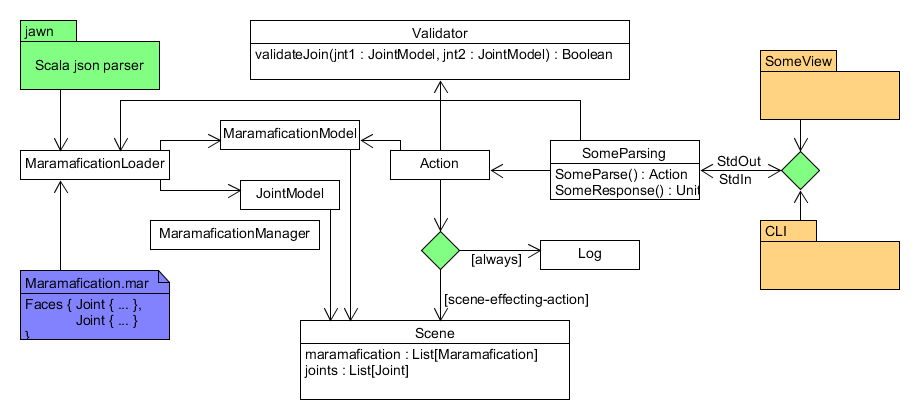
\includegraphics[width=\textwidth, height=\textheight, keepaspectratio]{architecture-marama-editor}
        \caption{The overview diagram of the marama-editor, used as blueprint in the early stages of development}
        \label{fig:ame}
    \end{figure}
    Figure \ref{fig:ame} shows the first prototype of the editor project.
    The idea was that the marama-editor would be a stand-alone terminal based program.
    This way it is easy for a seperate GUI project to attach itself to the editor, redirecting input and visualizing the state of the marama-editor.
    Now we encounter the entry point of the program.
    First some parsing has to be done, it looks for legal commands and fires the appropriate action, see:\ref{}.

    \begin{description}
        Actions
        \item[get maram] text
        \item[clear all] lorem ipsum
    \end{description}


    \subsection[Communication MVA-MEA]{Receiving command or information from MVA and MEA}
    \label{subsec:comchoice}
    In the ideal situation the Editor would be a command line tool for the Marama project.
    This way, it is easy to build a different, or more specialized view on top of the Editor.

    \subsection{Epics}
    \label{subsec:epics}
    The editor is made up of different epics.
    Epics are a collection of user stories that share a goal or functionality.

    \newcommand{\clickup}[1]{https://app.clickup.com/757520/761304/t/#1}

    \subsubsection{3D Camera Controls}
    \myparagraph{\href{\clickup{2e2ca}}{\#2e2ca} As a MGD or player I want to zoom in/out on the world when pinching}
    The camera zoom functionality is already implemented and enabled by libGDX on all supported devices (Desktop, Android).
    \myparagraph{\href{\clickup{2e2c1}}{\#2e2c1} As a MGD or player I want to rotate the camera by one-fingered swiping}
    The camera rotation functionality is already implemented and enabled by libGDX on all supported devices (Desktop, Android).

    \newpage
    %------------------------------------------------------------------------------------------------------------------------------------------------------- Build Automation
    \section{Continous Intergration}
    In this section build automation and its constituent components will be discussed.
    How we applied it, the software used and the targets and platforms supported are among a few.

    \newpage
    %------------------------------------------------------------------------------------------------------------------------------------------------------- References
    \bibliography{references}
    \bibliographystyle{ieeetr} % options: apalike for apa, ieeetr for ieee
\end{document}
